% Created by tikzDevice version 0.12.3.1 on 2021-01-13 20:53:15
% !TEX encoding = UTF-8 Unicode
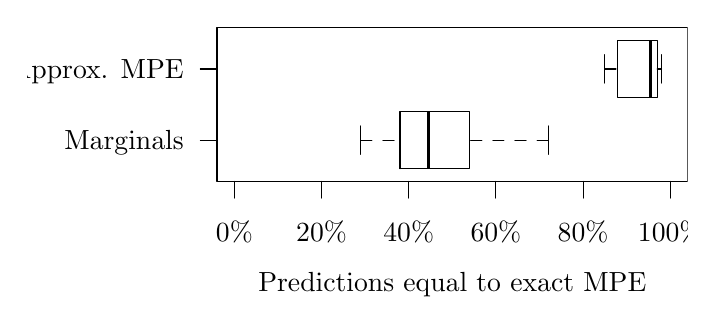
\begin{tikzpicture}[x=1pt,y=1pt]
\definecolor{fillColor}{RGB}{255,255,255}
\path[use as bounding box,fill=fillColor,fill opacity=0.00] (0,0) rectangle (238.49, 97.56);
\begin{scope}
\path[clip] ( 68.40, 42.00) rectangle (238.49, 97.56);
\definecolor{drawColor}{RGB}{0,0,0}

\path[draw=drawColor,line width= 1.2pt,line join=round] (144.78, 46.63) -- (144.78, 67.21);

\path[draw=drawColor,line width= 0.4pt,dash pattern=on 4pt off 4pt ,line join=round,line cap=round] (120.37, 56.92) -- (134.55, 56.92);

\path[draw=drawColor,line width= 0.4pt,dash pattern=on 4pt off 4pt ,line join=round,line cap=round] (188.09, 56.92) -- (159.75, 56.92);

\path[draw=drawColor,line width= 0.4pt,line join=round,line cap=round] (120.37, 51.78) -- (120.37, 62.06);

\path[draw=drawColor,line width= 0.4pt,line join=round,line cap=round] (188.09, 51.78) -- (188.09, 62.06);

\path[draw=drawColor,line width= 0.4pt,line join=round,line cap=round] (134.55, 46.63) --
	(134.55, 67.21) --
	(159.75, 67.21) --
	(159.75, 46.63) --
	(134.55, 46.63);

\path[draw=drawColor,line width= 1.2pt,line join=round] (225.10, 72.35) -- (225.10, 92.93);

\path[draw=drawColor,line width= 0.4pt,dash pattern=on 4pt off 4pt ,line join=round,line cap=round] (208.57, 82.64) -- (213.29, 82.64);

\path[draw=drawColor,line width= 0.4pt,dash pattern=on 4pt off 4pt ,line join=round,line cap=round] (229.04, 82.64) -- (227.47, 82.64);

\path[draw=drawColor,line width= 0.4pt,line join=round,line cap=round] (208.57, 77.50) -- (208.57, 87.79);

\path[draw=drawColor,line width= 0.4pt,line join=round,line cap=round] (229.04, 77.50) -- (229.04, 87.79);

\path[draw=drawColor,line width= 0.4pt,line join=round,line cap=round] (213.29, 72.35) --
	(213.29, 92.93) --
	(227.47, 92.93) --
	(227.47, 72.35) --
	(213.29, 72.35);
\end{scope}
\begin{scope}
\path[clip] (  0.00,  0.00) rectangle (238.49, 97.56);
\definecolor{drawColor}{RGB}{0,0,0}

\path[draw=drawColor,line width= 0.4pt,line join=round,line cap=round] ( 68.40, 56.92) -- ( 68.40, 82.64);

\path[draw=drawColor,line width= 0.4pt,line join=round,line cap=round] ( 68.40, 56.92) -- ( 62.40, 56.92);

\path[draw=drawColor,line width= 0.4pt,line join=round,line cap=round] ( 68.40, 82.64) -- ( 62.40, 82.64);

\node[text=drawColor,anchor=base east,inner sep=0pt, outer sep=0pt, scale=  1.00] at ( 56.40, 53.48) {Marginals};

\node[text=drawColor,anchor=base east,inner sep=0pt, outer sep=0pt, scale=  1.00] at ( 56.40, 79.20) {Approx. MPE};

\path[draw=drawColor,line width= 0.4pt,line join=round,line cap=round] ( 68.40, 42.00) --
	(238.49, 42.00) --
	(238.49, 97.56) --
	( 68.40, 97.56) --
	( 68.40, 42.00);

\path[draw=drawColor,line width= 0.4pt,line join=round,line cap=round] ( 74.70, 42.00) -- (232.19, 42.00);

\path[draw=drawColor,line width= 0.4pt,line join=round,line cap=round] ( 74.70, 42.00) -- ( 74.70, 36.00);

\path[draw=drawColor,line width= 0.4pt,line join=round,line cap=round] (106.20, 42.00) -- (106.20, 36.00);

\path[draw=drawColor,line width= 0.4pt,line join=round,line cap=round] (137.70, 42.00) -- (137.70, 36.00);

\path[draw=drawColor,line width= 0.4pt,line join=round,line cap=round] (169.19, 42.00) -- (169.19, 36.00);

\path[draw=drawColor,line width= 0.4pt,line join=round,line cap=round] (200.69, 42.00) -- (200.69, 36.00);

\path[draw=drawColor,line width= 0.4pt,line join=round,line cap=round] (232.19, 42.00) -- (232.19, 36.00);

\node[text=drawColor,anchor=base,inner sep=0pt, outer sep=0pt, scale=  1.00] at ( 74.70, 20.40) {0\%};

\node[text=drawColor,anchor=base,inner sep=0pt, outer sep=0pt, scale=  1.00] at (106.20, 20.40) {20\%};

\node[text=drawColor,anchor=base,inner sep=0pt, outer sep=0pt, scale=  1.00] at (137.70, 20.40) {40\%};

\node[text=drawColor,anchor=base,inner sep=0pt, outer sep=0pt, scale=  1.00] at (169.19, 20.40) {60\%};

\node[text=drawColor,anchor=base,inner sep=0pt, outer sep=0pt, scale=  1.00] at (200.69, 20.40) {80\%};

\node[text=drawColor,anchor=base,inner sep=0pt, outer sep=0pt, scale=  1.00] at (232.19, 20.40) {100\%};

\node[text=drawColor,anchor=base,inner sep=0pt, outer sep=0pt, scale=  1.00] at (153.45,  2.40) {Predictions equal to exact MPE};
\end{scope}
\end{tikzpicture}
